\chapter{The razor variables}
The top partners are particles with a large mass. Therefore the energy scale
of the events featuring a \TP is completely different with respect to
Standard Model processes. Many studies have been devoted during the course
of the last years to the development of kinematical variables that assist
the discovery of new physics~\cite{rogan_variables}.

We now introduce the relevant variables, and discuss their application to
our signal, which requires new techniques with respect to the standard
treatment of these variables.

\section{The variable $M_R$}
The razor variables were first introduced in the searches for supersymmetric
particles~\cite{supersimmetry_razor}. The simplest events in these searches
feature the pair production of two heavy supersymmetric particles. Each of
these particles decay to a SM particle, which is detected and measured, and
a non-interacting \emph{lightest supersymmetric particle} which escapes
detection and gives rise to \met (figure~\ref{fig:standard_razor_susy}).

\begin{figure}[htb]
    \centering
    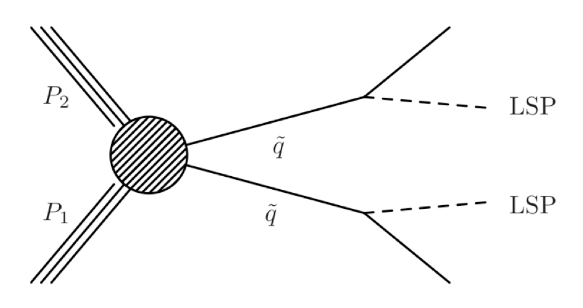
\includegraphics[width=.7/textwidth]{images/pdf/standard_razor_susy}

    \caption{Simple example of a supersymmetric event, with two heavy
    pair-produced SUSY particles, two invisible lightest supersymmetric
particles and two visible SM particles.}
    \label{fig:standard_razor_susy}
\end{figure}

In this kind of events, there is an additional, well-motivated approximation
that can be made. If the mass of the heavy particle is sufficiently large
relative to the collider energy $\sqrt{s}$, the particles will be mostly
produced near the threshold $\sqrt{\hat s} \approx 2M$, where
$\sqrt{\hat s}$ is the usual Mandelstam variable describing the hard
partonic process.
In this approximation, we can move from the laboratory reference frame to
the centre-of-mass frame of the pair-produced particles by finding the frame
where the magnitude of the momenta $\vec a$ and $\vec b$ of the visible particles are equal. This
frame is called the \emph{R frame}.
We define the R-frame mass $M_R$ as:
\begin{equation*}
            M_R = \sqrt{(a^0 - b^0)^2 - (a^3 + b^3)^2}
\end{equation*}
Where $a^\mu$ and $b^\mu$ are the four momenta of the visible particles, as
measured in the laboratory frame.
This quantity is invariant under longitudinal boosts, and has a distribution
peaked at the value of the massive particle.
